\documentclass[lettersize,journal]{IEEEtran}
\usepackage{amsmath,amsfonts}
\usepackage{algorithmic}
\usepackage{algorithm}
\usepackage{array}
\usepackage[caption=false,font=normalsize,labelfont=sf,textfont=sf]{subfig}
\usepackage{textcomp}
\usepackage{stfloats}
\usepackage{url}
\usepackage{verbatim}
\usepackage{graphicx}
\usepackage{cite}
\hyphenation{op-tical net-works semi-conduc-tor IEEE-Xplore}
% updated with editorial comments 8/9/2021

\begin{document}

\title{Distributed Formation Control for a Four-UAV Capture Net With Prescribed Plane Orientation}

% IEEE Publication Technology,~\IEEEmembership{Staff,~IEEE,}

\author{...}

% The paper headers
\markboth{Draft Manuscript}%
{Zhu: Distributed Formation Control for a Four-UAV Capture Net}

% \IEEEpubid{0000--0000/00\$00.00~\copyright~2021 IEEE}
% Remember, if you use this you must call \IEEEpubidadjcol in the second
% column for its text to clear the IEEEpubid mark.

\maketitle

\begin{abstract}
This paper studies the formation control problem of a four-UAV capture-net system operating in 3-D space. The four UAVs are treated as the vertices of an elastic net, and the desired capture configuration is described by local angle constraints, selected distance constraints, a plane-normal constraint, and a coplanarity constraint. A distributed control framework with disturbance-observer-based compensation is formulated to achieve the desired square net shape, regulate the plane orientation, maintain coplanarity, and track a desired common velocity in the presence of lumped disturbances. The proposed formulation provides a basis for the subsequent controller design, stability analysis, and simulation validation.
\end{abstract}

\begin{IEEEkeywords}
Capture net, formation control, UAVs, angle constraints, coplanarity control, disturbance observer.
\end{IEEEkeywords}

\section{Introduction}
\IEEEPARstart{M}{ulti-UAV} formation control has been widely studied because a coordinated group can perform tasks that are difficult for a single vehicle, such as cooperative transportation, search and rescue, and aerial manipulation. Compared with position-based and displacement-based methods, local sensing-based formation control reduces the dependence on global positioning and common reference frames. In this direction, bearing- and angle-based methods are especially attractive since relative direction information can be obtained from onboard vision or line-of-sight sensors.

Angle-rigidity-based formation control has been developed to stabilize formations using local angle measurements \cite{chen2021angleRigidity}. Since angle constraints are invariant under translation, rotation, and scaling, additional information is generally required when the scale or orientation of a formation must be prescribed. Recent studies have therefore introduced distance, orientation, or leader information to remove the ambiguity of angle-constrained formations \cite{chen2022stabilizing,chen2023angleConstrained,li2025localInfo}. For UAV systems operating in realistic environments, external disturbances and unmodeled effects can further degrade formation accuracy, which motivates the use of observer-based compensation schemes \cite{wang2025esoMultiUAV,ren2026observer}.

This paper considers a four-UAV capture-net formation in 3-D space. The UAVs form the four vertices of an elastic net, and the desired configuration is described by a square-shape constraint, a scale constraint, a plane-normal constraint, and a coplanarity constraint. The main objective is to develop a distributed formation controller with disturbance compensation such that the capture net maintains the desired planar square configuration while tracking a prescribed common velocity.

% \section{The Design, Intent, and \\ Limitations of the Templates}
\section{Problem Formulation}

Consider a group of four UAVs carrying an elastic capture net in 3-D space. The UAVs constitute the four vertices of the net and are indexed by
\begin{equation}
\label{eq:vertex-set}
\mathcal V=\{1,2,3,4\}.
\end{equation}
The position and velocity of agent \(i\) are denoted by \(p_i(t)\in\mathbb R^3\) and \(v_i(t)\in\mathbb R^3\), respectively. Unless otherwise stated, all vectors are expressed in a fixed inertial frame. Let
\begin{equation}
\label{eq:stacked-position}
p=\left[p_1^T,p_2^T,p_3^T,p_4^T\right]^T\in\mathbb R^{12}.
\end{equation}

\subsection{Agent Dynamics and Disturbance Model}

Each UAV is modeled as a double integrator. In the presence of system uncertainties, unmodeled dynamics, and external disturbances, agent \(i\) is governed by
\begin{equation}
\label{eq:agent-dynamics}
\begin{aligned}
\dot p_i(t)&=v_i(t),\\
\dot v_i(t)&=u_i(t)+f_i(t)+d_i(t),
\end{aligned}
\qquad i\in\mathcal V,
\end{equation}
where \(u_i(t)\in\mathbb R^3\) is the control input, \(f_i(t)\in\mathbb R^3\) denotes the system uncertainty and unmodeled dynamics, and \(d_i(t)\in\mathbb R^3\) denotes the external disturbance. The net-tension force is included in \(d_i(t)\). Define the lumped disturbance as
\begin{equation}
\label{eq:lumped-disturbance}
D_i(t)=f_i(t)+d_i(t).
\end{equation}
Then \eqref{eq:agent-dynamics} can be rewritten as
\begin{equation}
\label{eq:compact-dynamics}
\begin{aligned}
\dot p_i(t)&=v_i(t),\\
\dot v_i(t)&=u_i(t)+D_i(t),
\end{aligned}
\qquad i\in\mathcal V.
\end{equation}
For subsequent disturbance compensation, let \(\hat D_i(t)\) be the estimate of \(D_i(t)\) generated by a disturbance observer. The corresponding estimation error is defined as
\begin{equation}
\label{eq:disturbance-error}
\tilde D_i(t)=\hat D_i(t)-D_i(t).
\end{equation}
The observer structure will be specified in the control design section.

We impose the following assumptions to make the desired formation configuration attainable.

\emph{Assumption 1:} Each UAV is equipped with LOS sensing to acquire the relative direction information required by the formation controller.

\emph{Assumption 2(doubt):} Each UAV has access to the desired common velocity and the desired plane-normal direction expressed in its local coordinate frame.

\emph{Assumption 3:} The initial formation lies in a neighborhood of the desired configuration, and the positions of the agents are distinct and noncollinear.

\emph{Assumption 4:} For each \(i\in\mathcal V\), the lumped disturbance \(D_i(t)\) and its derivative \(\dot D_i(t)\) are bounded, i.e., there exist positive constants \(\bar D_i\) and \(\bar d_i\) such that
\begin{equation}
\label{eq:disturbance-bound}
\|D_i(t)\|\le \bar D_i,\qquad
\|\dot D_i(t)\|\le \bar d_i.
\end{equation}
Here, \(D_i(t)\) includes environmental disturbances, unmodeled dynamics, and the net-tension force acting on UAV \(i\).

\subsection{Desired Capture-Net Configuration}

For any \(i,j\in\mathcal V\), define the relative position, inter-agent distance, and bearing vector as
\begin{equation}
\label{eq:bearing-definition}
q_{ij}=p_j-p_i,\qquad
d_{ij}=\|q_{ij}\|,\qquad
b_{ij}=\frac{q_{ij}}{\|q_{ij}\|}.
\end{equation}
Under Assumption 1, agent \(i\) has access to the local bearing vectors \(b_{ij}\) and \(b_{ik}\). The interior angle formed by agents \(j\), \(i\), and \(k\) is given by
\begin{equation}
\label{eq:angle-definition}
\alpha_{jik}=\arccos\left(b_{ij}^{T}b_{ik}\right),
\qquad \alpha_{jik}\in[0,\pi].
\end{equation}

The in-plane square shape of the capture net is encoded by the angle constraint set
\begin{equation}
\label{eq:angle-set}
\mathcal A=\{(2,1,4),(3,2,1),(4,3,2),(1,4,3)\}.
\end{equation}
Each tuple \((j,i,k)\in\mathcal A\) represents the interior angle with UAV \(i\) as the vertex. For the desired square capture net, the desired angle is set to
\begin{equation}
\label{eq:desired-angle}
\alpha_{jik}^*(t)=\frac{\pi}{2},
\qquad (j,i,k)\in\mathcal A.
\end{equation}
The angle constraints characterize the desired square shape but do not determine the formation scale, since angles are invariant under translations, rotations, and scalings. To prescribe the scale while retaining the bearing/angle-based description, introduce the distance-constrained edge set
\begin{equation}
\label{eq:distance-edge-set}
\mathcal E_d=\{(1,2),(1,4)\}.
\end{equation}
Together with the right-angle constraints in \(\mathcal A\), these two distance constraints determine the side length of the square net locally \cite{li2025localInfo}. The desired distances satisfy
\begin{equation}
\label{eq:desired-distance}
d_{ij}=d_{ij}^*(t),
\qquad
(i,j)\in\mathcal E_d,
\end{equation}
where \(d_{ij}^*(t)=\ell^*\), and \(\ell^*>0\) denotes the desired side length of the capture net.

Since the capture net evolves in 3-D space, the in-plane angle and distance constraints alone do not prescribe the spatial orientation of the net plane. We use the plane formed by UAVs 1, 4, and 2 as the reference plane of the current formation. Its normal vector is
\begin{equation}
\label{eq:normal-142}
n_{142}=\frac{b_{14}\times b_{12}}
{\|b_{14}\times b_{12}\|}.
\end{equation}
For a capture net, the two sides of the net plane are physically equivalent. Thus, \(n_d\) and \(-n_d\) represent the same desired capture plane. Define the unoriented desired normal set as
\begin{equation}
\label{eq:normal-set}
\mathcal N_d=\{n_d,-n_d\},
\qquad \|n_d\|=1,
\end{equation}
and select the representative element closest to the current normal direction as
\begin{equation}
\label{eq:normal-representative}
\bar n_d=\operatorname*{arg\,max}_{\eta\in\mathcal N_d}
\left(n_{142}^{T}\eta\right).
\end{equation}
The normal-direction error is defined by
\begin{equation}
\label{eq:normal-error}
e_n=n_{142}\times \bar n_d.
\end{equation}
When \(e_n=0\), one has \(n_{142}=n_d\) or \(n_{142}=-n_d\), i.e., the current net plane is aligned with the desired capture plane in an unoriented sense.

The remaining vertex UAV 3 is then required to follow the reference plane so that the four UAVs form a physically planar net. Define the coplanarity error of UAV 3 with respect to the reference plane as
\begin{equation}
\label{eq:coplanar-error}
e_{\mathrm{cop}}=b_{13}^{T}n_{142}.
\end{equation}
As illustrated in Fig.~\ref{fig:coplanar_constraint}, \(e_{\mathrm{cop}}=0\) implies that UAV 3 lies on the plane determined by UAVs 1, 4, and 2. Hence, the four UAVs are coplanar.

\begin{figure}[!t]
\centering
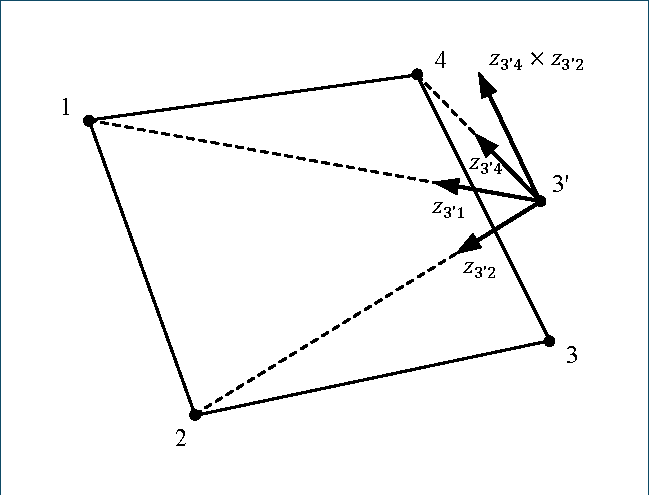
\includegraphics[width=2.5in,trim=2pt 2pt 2pt 2pt,clip]{figures/fig_1}
\caption{Coplanarity constraint of UAV 3 with respect to the reference plane formed by UAVs 1, 4, and 2.}
\label{fig:coplanar_constraint}
\end{figure}

Combining the above constraints, the desired capture-net configuration set is defined as
\begin{equation}
\label{eq:desired-formation-set}
\begin{aligned}
\mathcal S(\ell^*,n_d)=\{p\in\mathbb R^{12}\mid{}&
\alpha_{jik}=\alpha_{jik}^*(t),\quad d_{ij}=d_{ij}^*(t),\\
&
e_{\mathrm{cop}}=0,\quad n_{142}=\bar n_d\}.
\end{aligned}
\end{equation}
Here, the angle and distance constraints are imposed for all \((j,i,k)\in\mathcal A\) and \((i,j)\in\mathcal E_d\), respectively. The set \(\mathcal A\) specifies the square shape, \(\mathcal E_d\) fixes the scale, \(e_{\mathrm{cop}}\) enforces coplanarity, and \(n_{142}=\bar n_d\) prescribes the plane orientation.

The following sensing assumption is imposed to obtain the required scale information.

\emph{Assumption 5:} Only UAV 1 measures the distances to its two neighboring UAVs, namely \(d_{12}\) and \(d_{14}\), and the measured distances can be transmitted to the corresponding neighboring UAVs when needed.

\subsection{Control Objective}

\emph{Problem 1:} Consider the four-UAV system \eqref{eq:compact-dynamics} under Assumptions 1--5. Design a distributed formation controller and a disturbance-observer-based compensation mechanism such that, despite system uncertainties, external disturbances, and the equivalent rope-tension effect, the UAVs form and maintain the desired planar square capture net in 3-D space. In addition, the net plane should align with the desired unoriented normal direction, and all UAVs should track a desired common velocity. The formation maneuvering objective consists of planar square-shape control, plane-normal control, and velocity tracking.

For initial conditions in a neighborhood of \(\mathcal S(\ell^*,n_d)\), the closed-loop formation maneuvering objective can be described as follows:
\begin{align}
\lim_{t\to+\infty}
\left(\alpha_{jik}(t)-\alpha_{jik}^*(t)\right)&=0,
& (j,i,k)&\in\mathcal A, \label{eq:angle-convergence}\\
\lim_{t\to+\infty}
\left(d_{ij}(t)-d_{ij}^*(t)\right)&=0,
& (i,j)&\in\mathcal E_d, \label{eq:distance-convergence}\\
\lim_{t\to+\infty}e_{\mathrm{cop}}(t)&=0, \label{eq:coplanar-convergence}\\
\lim_{t\to+\infty}e_n(t)&=0, \label{eq:normal-convergence}\\
\lim_{t\to+\infty}
\left(v_i(t)-v_c^*(t)\right)&=0,
& i&\in\mathcal V, \label{eq:velocity-convergence}
\end{align}
where \(v_c^*(t)\) denotes the desired common velocity.


% \section{Where to Get \LaTeX \ Help --- User Groups}
\section{Main Results}
In this section, we introduce the distributed formation control law and the disturbance-observer-based compensation scheme for the four-UAV capture-net formation. First, the formation controller is constructed to regulate the planar square shape, the plane-normal direction, the coplanarity error, and the common velocity tracking error. Next, geometric interpretations of the plane-normal control and the coplanarity control are provided to clarify how the capture-net plane is oriented and maintained. Finally, the stability of the closed-loop system is analyzed under the assumptions stated in Section~II.

\section{Simulations}
In this section, numerical simulations will be carried out to validate the proposed formation control scheme. The simulation scenario considers four UAVs connected by an elastic capture net and moving in 3-D space under bounded lumped disturbances. The desired formation is selected as a square net with side length \(\ell^*\), prescribed unoriented normal direction \(n_d\), and desired common velocity \(v_c^*(t)\).

The simulation results are expected to demonstrate the convergence of the angle errors, distance errors, coplanarity error, normal-direction error, and velocity tracking errors. In particular, the angle and distance responses verify the regulation of the planar square shape and scale, while the responses of \(e_{\mathrm{cop}}\) and \(e_n\) show that the four UAVs become coplanar and that the net plane aligns with the desired capture plane. The disturbance observer is evaluated by comparing the lumped disturbance \(D_i(t)\) and its estimate \(\hat D_i(t)\), thereby illustrating the compensation effect on the closed-loop formation performance.

\section{Conclusion and Discussion}
This paper formulated a distributed formation control problem for a four-UAV capture-net system in 3-D space. The desired capture-net configuration was described by local angle constraints, selected distance constraints, a plane-normal constraint, and a coplanarity constraint. Based on this formulation, a disturbance-observer-based control framework was introduced to achieve square-shape regulation, scale assignment, plane-orientation control, coplanarity maintenance, and common-velocity tracking in the presence of lumped disturbances.

Future work will focus on completing the experimental validation of the proposed controller, incorporating a more detailed net-tension model, and extending the method to capture nets with more vertices. The effects of sensing noise, communication delay, and actuator saturation also deserve further investigation.

\begin{thebibliography}{1}
\bibliographystyle{IEEEtran}

\bibitem{chen2021angleRigidity}
L. Chen, M. Cao, and C. Li, ``Angle rigidity and its usage to stabilize multiagent formations in 2-D,'' \textit{IEEE Trans. Autom. Control}, vol. 66, no. 8, pp. 3667--3681, Aug. 2021, doi: 10.1109/TAC.2020.3025539.

\bibitem{chen2022stabilizing}
L. Chen, Q. Yang, M. Shi, Y. Li, and M. Feroskhan, ``Stabilizing angle rigid formations with prescribed orientation and scale,'' \textit{IEEE Trans. Ind. Electron.}, vol. 69, no. 11, pp. 11654--11665, Nov. 2022, doi: 10.1109/TIE.2021.3120476.

\bibitem{chen2023angleConstrained}
L. Chen, J. Xiao, R. C. H. Lin, and M. Feroskhan, ``Angle-constrained formation maneuvering of unmanned aerial vehicles,'' \textit{IEEE Trans. Control Syst. Technol.}, vol. 31, no. 4, pp. 1733--1746, Jul. 2023, doi: 10.1109/TCST.2023.3240286.

\bibitem{li2025localInfo}
J. Li, L. Chen, and C. Li, ``Multi-agent distributed formation control using local information measurements,'' \textit{Sci. China Technol. Sci.}, vol. 68, no. 7, Art. no. 1720402, 2025, doi: 10.1007/s11431-024-2896-5.

\bibitem{wang2025esoMultiUAV}
R. Wang, T. Mei, W. Ma, and W. Hao, ``Disturbance rejection control for multi-UAV formations based extended state observer,'' in \textit{Proc. 40th Youth Acad. Annu. Conf. Chin. Assoc. Autom.}, 2025, pp. 2144--2149, doi: 10.1109/YAC66630.2025.11150314.

\bibitem{ren2026observer}
W. Ren, G.-R. Duan, P. Li, and H. Kong, ``Observer-based active fault/disturbance compensation control for fully actuated systems,'' \textit{Sci. China Inf. Sci.}, vol. 69, no. 5, Art. no. 152202, 2026, doi: 10.1007/s11432-025-4817-2.

\end{thebibliography}

\end{document}
